% ОБЯЗАТЕЛЬНО ИМЕННО ТАКОЙ documentclass!
% (Основной кегль = 14pt, поэтому необходим extsizes)
% Формат, разумеется, А4
% article потому что стандарт не подразумевает разделов
% Глава = section, Параграф = subsection
% (понятия "глава" и "параграф" из документа, описывающего диплом)
\documentclass[a4paper,article,14pt]{extarticle}

% Подключаем главный пакет со всем необходимым
\usepackage{spbudiploma_tempora}

% Пакеты по желанию (самые распространенные)
% Хитрые мат. символы
\usepackage{euscript}
% Таблицы
\usepackage{longtable}
\usepackage{makecell}
% Картинки (можно встявлять даже pdf)
\usepackage[pdftex]{graphicx}
\usepackage{adjustbox}

\usepackage{amsthm,amssymb, amsmath}
\usepackage{textcomp}

\usepackage{longtable}
\usepackage{floatrow} % Подключаем пакет floatrow


\begin{document}

% Титульник (ВКР) в файле title.tex
% --------------------- Титульник ВКР СПбГУ -----------------------------
% Автор: Тоскин Николай, itonik@me.com
% Если заметили ошибку, напишите на email
% Если хотите добавить изменение самостоятельно:
% https://github.com/itonik/spbu_diploma/
% Использованы материалы:
% habr.com/ru/post/144648/
% cpsconf.ru
% Документы ниже могут уже быть неактуальны, тем не менее за годы ничего
% нового не появилось
% Текст:
% http://edu.spbu.ru/images/data/normativ_acts/local/20181030_10432_1.pdf
% Титульный лист:
% http://edu.spbu.ru/images/data/normativ_acts/local/20180703_6616_1.pdf
% -----------------------------------------------------------------------

% Титульный лист диплома СПбГУ
% Временное удаление foot на titlepage
\newgeometry{left=30mm, top=20mm, right=15mm, bottom=20mm, nohead, nofoot}
\begin{titlepage}
\begin{center}

\textbf{Санкт--Петербургский}
\textbf{государственный университет}

\vspace{35mm}

\textbf{\textit{\large Тарасов Даниил Антонович}} \\[8mm]
% Название
\textbf{\large Научно-исследовательская работа}\\[3mm]
\textbf{\textit{\large Исследование систем видеоконференций}}

\vspace{20mm}
Уровень образования: бакалавриат\\
Направление 02.03.02 «Фундаментальная информатика и информационные технологии»\\
Основная образовательная программа СВ.5003.2021
«Программирование и информационные технологии»\\[25mm]


% Научный руководитель, рецензент
\begin{flushright}
\begin{minipage}[t]{0.65\textwidth}
{Научный руководитель:} \\
доцент, кафедра компьютерного моделирования и многопроцессорных систем \\ и систем, к.ф. - м.н. Корхов~Владимир Владиславович

\vspace{10mm}

% {Рецензент:} \\
% профессор, кафедра компьютерных технологий \\и систем, д.ф. - м.н. Веремей~Евгений Игоревич
\end{minipage}
\end{flushright}

\vfill 

{Санкт-Петербург}
\par{\the\year{} г.}
\end{center}
\end{titlepage}
% Возвращаем настройки geometry обратно (то, что объявлено в преамбуле)
\restoregeometry
% Добавляем 1 к счетчику страниц ПОСЛЕ titlepage, чтобы исключить 
% влияние titlepage environment
\addtocounter{page}{1}


% Содержание
\tableofcontents
\pagebreak

% Introduction в файле intro.tex
\specialsection{Введение}

В настоящее время системы видеоконференций являются неотъемлемой частью повседневной коммуникации. Развитие технологии связи привели к появлению различных платформ и технологии, обеспечивающих возможность удаленного общения. Среди них немаловажное место занимает фреймворк WebRTC (Web Real-Time Communication), который позволяет осуществлять передачу аудио и видеоданных в реальном времени через веб-браузер без необходимости установки дополнительного программного обеспечения.

В рамках данной научной исследовательской работы мы рассмотрим историю развития систем видеоконференций, обоснуем выбор WebRTC в контексте современных требований и ожиданий пользователей. Кроме того, мы рассмотрим основные проблемы, с которыми сталкиваются разработчики систем видеоконференций и варианты их решения.

\pagebreak

% History в файле history.tex
\specialsection{История}

История систем видеоконференций началась в 1920-ых годах, когда появились первые стабильные и работающие телекамеры, тогда же компания AT&T Bell Telephone Laboratories создала работающий комплекс телефонной связи, которые транслировал изображение на расстояние 200 миль. В 1930-ых та же компания AT&T продемонстрировала сеанс двусторонней видеосвязи между офисами AT&T на Манхэттене, однако затянувшиеся последствия Великой депрессии затормозили развитие видеосвязи.

В 1980-ых компания Compression Labs составила конкуренцию AT&T и выпутила CLI T1 в качестве первой коммерческой системы групповой видеоконфенцсвязи. Ее первоначальная стоимость составляла 250000 долларов, а каждый звонок стоил 1000 долларов в час.

В 1990-ых произошел Бум Интернета и развития цифровой телефонии. В 1991 году студенты факультета компьютерных наук Кембриджского университета изобрели первую веб-камеру.

В начале 2000-ых появились смартфоны, оснащенные камерами на задней и передней панелях для съемки фотографий. Три эстонских инженера-программиста представили Skype в августе 2003 года. Два бывших сотрудника Yahoo основали WhatsApp в 2009 году как приложение для мгновенного обмена сообщениями. В 2020-ых блокировка COVID-19 заставило многих людей по всему миру работать из дома, что привело к буму на все видеоустройства и большой популярности систем видеоконференций \cite{v1}.

\pagebreak

% Why WebRTC? в файле why_webrtc.tex
\specialsection{Почему WebRTC?}

Инициатива WebRTC достигла впечатляющих результатов с точки зрения промышленного интереса, проникновения технологии в устройства конечных пользователей и постоянно растущего сообщества разработчиков. Сегодня WebRTC поддерживается основными мобильными платформами и интернет-браузерами, позволяя потенциально миллиардам пользователей беспрепятственно устанавливать сеансы связи в режиме реального времени \cite{v2}.

Кратко рассмотрим ключевые особенности WebRTC:
\begin{itemize}
	\item[--] Открытый стандарт;
	\item[--] Разные реализации;
	\item[--] Доступность в браузерах;
        \item[--] Обязательное шифрование;
        \item[--] Отображение NAT (NAT Traversal);
        \item[--] Перепрофилирование существующих технологий;
        \item[--] Контроль перегрузки (congestion control);
        \item[--] Низкая задержка (на уровне долей секунды, sub-second latency) \cite{v3}.
\end{itemize}

\pagebreak


% WebRTC в файле webrtc.tex
\section{WebRTC}

Рассмотрим WebRTC более подробно. WebRTC (Web Real-Time \\ Communication) -- коммуникация в режиме реального времени) -- это набор правил, позволяющий двум агентам вести двунаправленную безопасную коммуникацию в режиме реального времени.

\begin{figure}[ht]
\begin{center}
\scalebox{0.5}{
   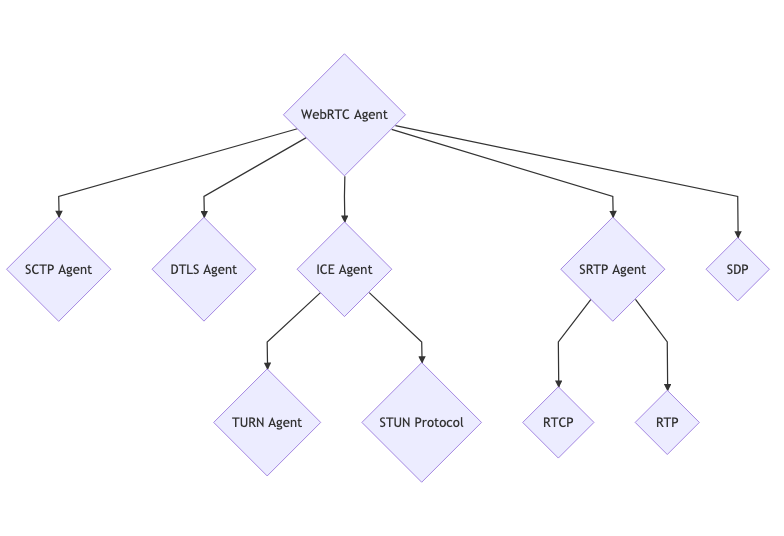
\includegraphics{images/webrtc_orchestr.png}
}

\caption{
\label{webrtc-orchestrator}
     WebRTC - оркестратор}
\end {center}
\end {figure}

Фактически WebRTC -- это оркестратор нескольких других протоколов, Рисунок ~\ref{webrtc-orchestrator}.

В процессе установки соединения можно выделить 4 основных этапа:
\begin{itemize}
	\item[--] Сигнализация;
	\item[--] Подключение;
        \item[--] Безопасность;
        \item[--] Коммуникация \cite{v3}.
\end{itemize}

Далее рассмотрим эти 4 этапа.

\subsection{Сигнализация}

Сигнализация -- это подготовка к совершению звонка. После обмена необходимой информацией участники могут общаться друг с другом напрямую.

Для совершения этого этапа WebRTC используется протокол SDP. Он позволяет двум участникам обменяться состоянием, необходимым для установки соединения. Протокол описания сессии определен в RFC 8866. Описание сессии представляет собой описание медиа (media description) и состоит из пар ключ/значение \cite{v21}.

\subsection{Подключение}

В WebRTC используется P2P (Peer-to-Peer) архитектура. Задача WebRTC обеспечить возможность двунаправленной коммуникации между двумя участниками.

ICE -- это протокол, который определяет наилучший способ для установки соединения между двумя участниками. Каждый участник определяет путь, по которому он может быть достигнут, затем ICE выбирает наиболее подходящую пару путей \cite{v22}.

\subsection{Безопасность}

Каждое соединения WebRTC аутентифицируется и шифруется. Таким образом, мы можем быть уверены, что третья сторона не видит того, что мы отправляем, и не может добавлять свои сообщения.

Для обеспечения безопасности соединения WebRTC использует DTLS и SRTP протоколы.

DTLS позволяет выполнить подготовку сессии и безопасно обмениваться данными между пирами. DTLS -- это клиент-серверный протокол, поэтому одна из сторон должна инициировать рукопожатие, в ходе него каждая из сторон генерирует сертификат. После завершения рукопожатия каждый сертификат сравнивается с его хешем, содержащим описание сессии, все это позволяет убедиться, что рукопожатие произошло с ожидаемым участником.

SRTP был разработан для безопасного обмена медиаданными. Для создания сессии SRTP мы инициализируем ее с помощью ключей, сгенерированных DTLS. После установки соединения стороны могут обмениваться зашифрованными медиаданными \cite{v23}.

\subsection{Коммуникация}

Для обмена данными WebRTC предоставляет каналы. Между двумя участниками может быть 65534 каналов. По умолчанию он гарантирует сохранение порядка сообщений.

Канал данных -- это абстракция потоков, из которых состоит SCTP. SCTP -- это транспортный протокол, являющийся альтернативой TCP и UDP, он определен в RFC 4960. Все настройки, связанные с продолжительностью существования канала и порядком доставки сообщений, передаются агенту SCTP \cite{v24}.

\pagebreak

% Expectations в файле expectations.tex
\section{История}

История систем видеоконференций началась в 1920-ых годах, когда появились первые стабильные и работающие телекамеры, тогда же компания AT\&T Bell Telephone Laboratories создала работающий комплекс телефонной связи, которые транслировал изображение на расстояние 200 миль. В 1930-ых та же компания AT\&T продемонстрировала сеанс двусторонней видеосвязи между офисами AT\&T на Манхэттене, однако затянувшиеся последствия Великой депрессии затормозили развитие видеосвязи.

В 1980-ых компания Compression Labs составила конкуренцию AT\&T и выпутила CLI T1 в качестве первой коммерческой системы групповой видеоконфенцсвязи. Ее первоначальная стоимость составляла 250000 долларов, а каждый звонок стоил 1000 долларов в час.

В 1990-ых произошел Бум Интернета и развития цифровой телефонии. В 1991 году студенты факультета компьютерных наук Кембриджского университета изобрели первую веб-камеру.

В начале 2000-ых появились смартфоны, оснащенные камерами на задней и передней панелях для съемки фотографий. Три эстонских инженера-программиста представили Skype в августе 2003 года. Два бывших сотрудника Yahoo основали WhatsApp в 2009 году как приложение для мгновенного обмена сообщениями. В 2020-ых блокировка COVID-19 заставило многих людей по всему миру работать из дома, что привело к буму на все видеоустройства и большой популярности систем видеоконференций \cite{v1}.

\pagebreak

% Network problems в файле network_problems.tex
\section{Основные проблемы, влияющие на качество видеоконференций}

В современном мире на уровне сетевых коммуникаций возникают различные проблемы, влияющие на качество и надежность передачи данных, которые в конечном итоге могут негативно сказываться на качестве видеоконференций:
\begin{itemize}
	\item[--] Перегрузка сетей;
	\item[--] Потеря пакетов;
        \item[--] Пропускная способность сетей;
        \item[--] Jitter;
        \item[--] NAT;
        \item[--] MTU;
        \item[--] Reordering \cite{v4}.
\end{itemize}

Технология WebRTC представляет мощный набор инструментов, который способен решить эти проблемы, обеспечивая стабильное взаимодействие в реальном времени.

\subsection{Перегрузка сетей}

Одна из распространненых сетевых проблем -- перегрузка сетей, появляется, когда сетевой узел или линия связи переносит больше данных, чем может обрабатывать. Частые эффекты включают задержку в очереди, потерю пакетов или блокировку новых соединений, в худшем случае это может привести к снижению пропускной способности сети.

Для отслеживания и предотвращения перегрузки сетей существуют разные решения, например:
\begin{itemize}
	\item[--] Экспоненциальная выдержка -- это алгоритм, использующий обратную связь для мультипликативного уменьшения частоты некоторого процесса, чтобы постепенно, чтобы постепенно найти приемлимую частоту. Этот алгоритм обычно используется для планирования повторных отправок после коллизий. После первой коллизии каждый отправитель будет ждать 0 или 1 slot time. После второй коллизии отправители будут ждать где-то от 0 до 3 slot times включительно. По мере увеличения количества попыток повторной отправки число вариантов для задержки растет экспоненциально;
        \item[--] Приоритезация сетевых пакетов -- это метод, в котором пакеты, помеченные как "важные", пропускаются в первую очередь, а менее важные придерживаются, пока линия не освободится \cite{v11}.
\end{itemize}

\subsection{Потеря пакетов}

Потеря пакетов это частая проблема, которая характеризуется тем, что сообщения теряются при передаче, то есть не доходят до адресата. Для решения этой проблемы WebRTC предлагает несколько вариантов:
\begin{itemize}
	\item[--] Если были утеряны медиа-пакеты, то мы можем скрыть этот факт и восстановить пакеты самостоятельно, "догадываясь" о том, что было потеряно. Некоторые кодеки умеют восстанавливать потерянные кадры заменой их на тишину или путем повторения уже принятой речи, например, последнего кадра \cite{v8};
	\item[--] Retransmission (Ретрансляция) в случае, когда нас устраивают возникающие задержки, необходимые для запроса повторной отправки. Осуществляется RTP \cite{v9};
        \item[--] FEC (Forward Error Connection) -- это механизм, при котором медиапакета заранее дублируются и отправляются по сети несколько раз. Таким образом, даже если некоторые пакеты не будут получены, медиапоток все равно можно будет правильно разобрать и декодировать \cite{v10}.
\end{itemize}

\subsection{Пропускная способность сетей}

Начнем с определения пропускной способности сети -- это количество данных, которые можно передать по сети. Это динамическая величина, которая зависит от нагрузки, то есть от количества людей, использующих этот маршрут. Перегрузка сети в худшем случае может привести к потери пакетов, увеличению задержки и джиттера, что негативно сказывается на коммуникации в реальном времени.

Подход WebRTC заключается в том, чтобы попытаться оценить доступную пропускную способность сети и ограничить отправителя от отправки черезчур большего от нашей оценки. Оценка пропускной способности основана на эвристике, которая моделирует поведение сети и пытается его предугадать.

В WebRTC используются два основных подхода для оценки пропускной способности \cite{v5}:
\begin{itemize}
	\item[--] REMB \cite{v6};
	\item[--] transport-cc \cite{v7}.
\end{itemize}

\subsection{Jitter}

При отправке пакетов нет гарантии, что они будут доставлены в те же промежутки, с которыми были отправлены. Разница от ожидаемого интервала получения пакетов называется джиттером. Чем он выше, тем сильнее он влияет на качество передачи данных.

В виду того, что голос и видео чувствительны ко времени, при получении медиапакетов их необходимо собрать, переупорядочить и затем определять время, основываясь на последовательности и различиях, в которых они были сгенерированы, а не на последовательности и времени, в которых они были получены. Этим занимается буффер джиттера и в WebRTC имеется собственная реализация, которая учитывает задержку сети, любые наблюдаемые потери пакетов и "расстояние" между входящими аудио- и видеопакетами \cite{v12}.

\begin{figure}[ht]
\begin{center}
\scalebox{0.4}{
   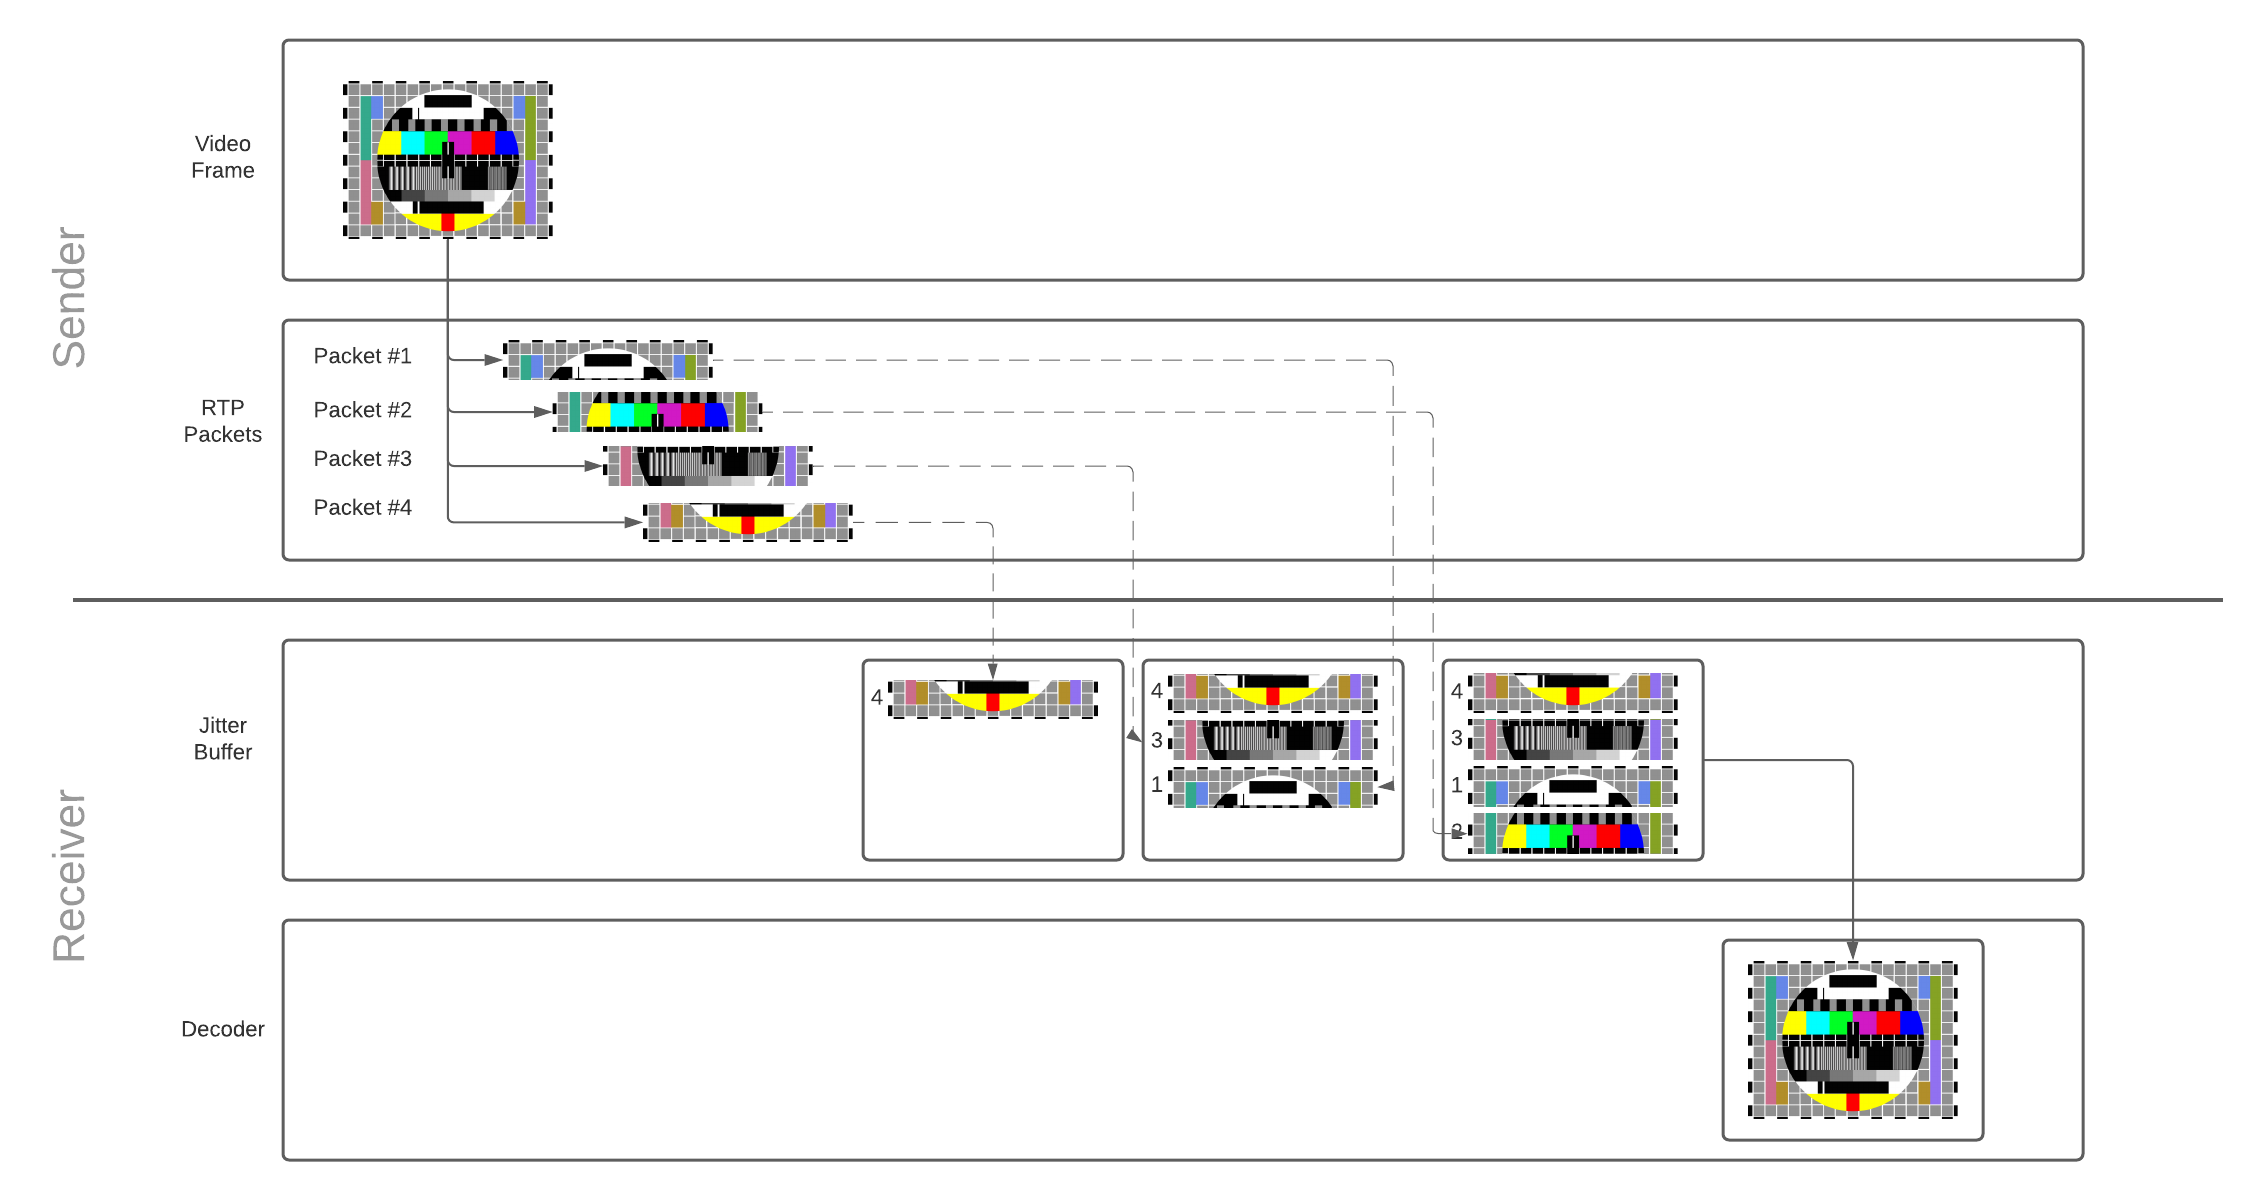
\includegraphics{images/jitter_buffer.png}
}

\caption{
\label{jitter-buffer}
     Джиттер буффер}
\end {center}
\end {figure}

Кратко алгоритм можно описать так, Рисунок ~\ref{jitter-buffer}:
\begin{itemize}
	\item[1.] Каждый пакет добавляется в буфер джиттера сразу после его получения;
	\item[2.] Как только пакетов становится достаточно для реконструкции кадра, пакеты, составляющие кадр, освобождаются из буфера и передаются для декодирования;
        \item[3.] Декодер, в свою очередь, декодирует и отрисовывает видеокадр на экране пользователя.
\end{itemize}

Поскольку буфер джиттера имеет ограниченную емкость, пакеты, которые остаются в буфере слишком долго, отбрасываются \cite{v13}.

\subsection{NAT}

NAT расшифровывается как трансляция сетевых адресов, обычно располагается между частной и публичной сетями и встроена в устройства сетевой маршрутизации. Входящий трафик в частную сеть направляется через привязку публичного адреса, которая возникает на устройстве NAT.

WebRTC должен иметь возможность передевать медиа между двумя абонентами, которые могут находиться за NAT устройствами, для этого необходимо, чтобы внешние пакеты могли проходить во внутреннюю сеть. STUN (Session Traversal Utilities for NAT) -- это стандартный метод обхода NAT, используемый в WebRTC \cite{v26}.

\begin{figure}[ht]
\begin{center}
\scalebox{0.5}{
   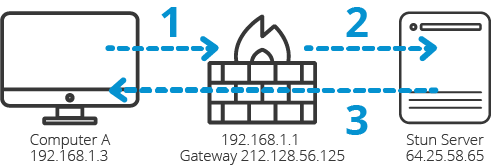
\includegraphics{images/stun.png}
}

\caption{
\label{stun}
     STUN}
\end {center}
\end {figure}


STUN-сервер позволяет своим клиентам находить публичный адрес, тип NAT, за которым они находятся и порт Интернета, связываемый NAT с конкретным локальным портом, Рисунок ~\ref{stun}. Затем эта информация используется WebRTC для настройки связи UDP между клиентами. Протокол STUN определяется стандартом RFC 3489 \cite{v25}.

\begin{figure}[ht]
\begin{center}
\scalebox{0.5}{
   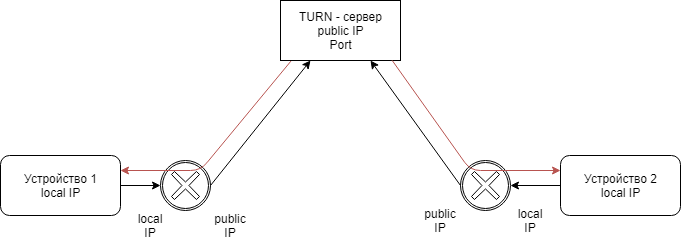
\includegraphics{images/turn.png}
}

\caption{
\label{turn}
     TURN}
\end {center}
\end {figure}

TURN (Traversal Using Relays around NAT) используется для передачи мультимедиа через сервер TURN, когда использование STUN невозможно. Решение о том, использовать STUN или TURN, принимается протоколом ICE. TURN-сервер фактически выступает проксирующим звеном между двумя клиентами, пропуская через себя весь трафик, Рисунок ~\ref{turn}.

ICE (Interactive Connection Establishment) -- это еще одно дополнение к протоколам STUN и TURN. Его задачи:
\begin{itemize}
	\item[--] Собрать данные об интерфейсах;
        \item[--] Проверить удаленные сервера STUN;
        \item[--] Проверить удаленные сервера TURN;
        \item[--] Проверить возможность установления соединения.
\end{itemize}

ICE выбирает самый легкий для прохождения маршрут (процедура номинирования пар) и выполняет проверку доступности между пиром и клиентом (могут ли они достучаться друг до друга). Приоритезация такая: без STUN сервера -- самый высокий приоритет, с использованием STUN -- пониже, с TURN -- самый низкий \cite{v27}.

\subsection{MTU}

MTU (Maximum Transmission Unit) -- это максимальный размер пакета, который может быть передан по сети. Если пакет передается с MTU большим, чем максимальный MTU на сети, то этот пакет фрагментируется. Конечно, он потом соберется обратно, однако если потеряется какая-то часть пакета, то потеряются все пакеты, поэтому необходимо оптимально работать с таким размером пакета, который соответствует MTU сети \cite{v4}.

WebRTC устанавливает размер MTU около 1200 байт и использует его для своих расчетов пакетирования (плюс-минус несколько байт). Использование такого значения гарантирует, что WebRTC будет хорошо работать в большинстве сетевых конфигураций \cite{v14}.

\subsection{Reordering}

Во время путешествия сетевых пакетов между источником и пунктом назначения есть вероятность переупорядочивания пакетов, то есть пакеты могут прибыть в другом порядке относительного того, в каком они были отправлены источником.

Для приложений видеоконференций, использующий протокол UDP и не использующих, например, метод коррекции ошибок вперед (FEC), переупорядочивание пакетов является проблемой, поскольку обычно приводит к потере данных, поскольку пакеты, приходящие не по порядку, отбрасываются, в худшем случае можно потерять целый видеокадр или аудиосегмент.

\begin{figure}[ht]
\begin{center}
\scalebox{0.6}{
   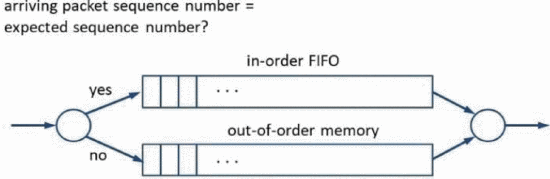
\includegraphics{images/out_of_order_memory.png}
}

\caption{
\label{out-of-order}
     Упорядочивающая архитектура с одной out-of-order памятью}
\end {center}
\end {figure}

Один из простейших методов коррекции переупорядочивания пакетов заключается в наличии памяти для неупорядоченных пакетов, в которой хранятся все пакеты, полученные с неожиданным порядковым номером. Эта память затем проверяется, когда ожидаемый номер не присутствует в конце очереди FIFO. Идея проиллюстрирована на Рисунке ~\ref{out-of-order}. Out-of-order буфер может быть организован как FIFO для простой коррекции переупорядочивания \cite{v15}.

\pagebreak

% Video в файле video.tex
\section{Передача видео}

Еще одна из важнейших проблем, решаемых WebRTC -- передача видео. Это сложный процесс, для хранения 30-минутного несжатого 720 8-битного видео требуется около 110 Гб. В таких условиях конференция с четырьмя участниками является невозможной. Для решения этой проблемы используют сжатие.

Сжатие делится на 2 типа:
\begin{itemize}
	\item[1.] Сжатие внутри кадра (intra-frame compression) -- это сжатие, которое уменьшает количество бит, используемых для описания единичного видеофрейма. Подобная техника используется для сжатия неподвижных изображений, например, JPEG;
	\item[2.] Межкадровое сжатие (inter-frame compression) -- способ не передавать одинаковую информацию дважды.
\end{itemize}

Кадры при межкадровом сжатии делятся на 3 типа:
\begin{itemize}
	\item[--] I-Frame -- полное изображение, которое может быть декодировано без каких-либо изменений;
	\item[--] P-Frame -- частичное изображение, содержащее только изменения предыдущего изображения;
        \item[--] B-Frame -- частичное изображение, представляющее собой модификацию предыдущего и последующего изображений.
\end{itemize}

Ниже приведена визуализация трех типов кадров, Рисунок ~\ref{frame-types}.

\begin{figure}[ht]
\begin{center}
\scalebox{0.15}{
   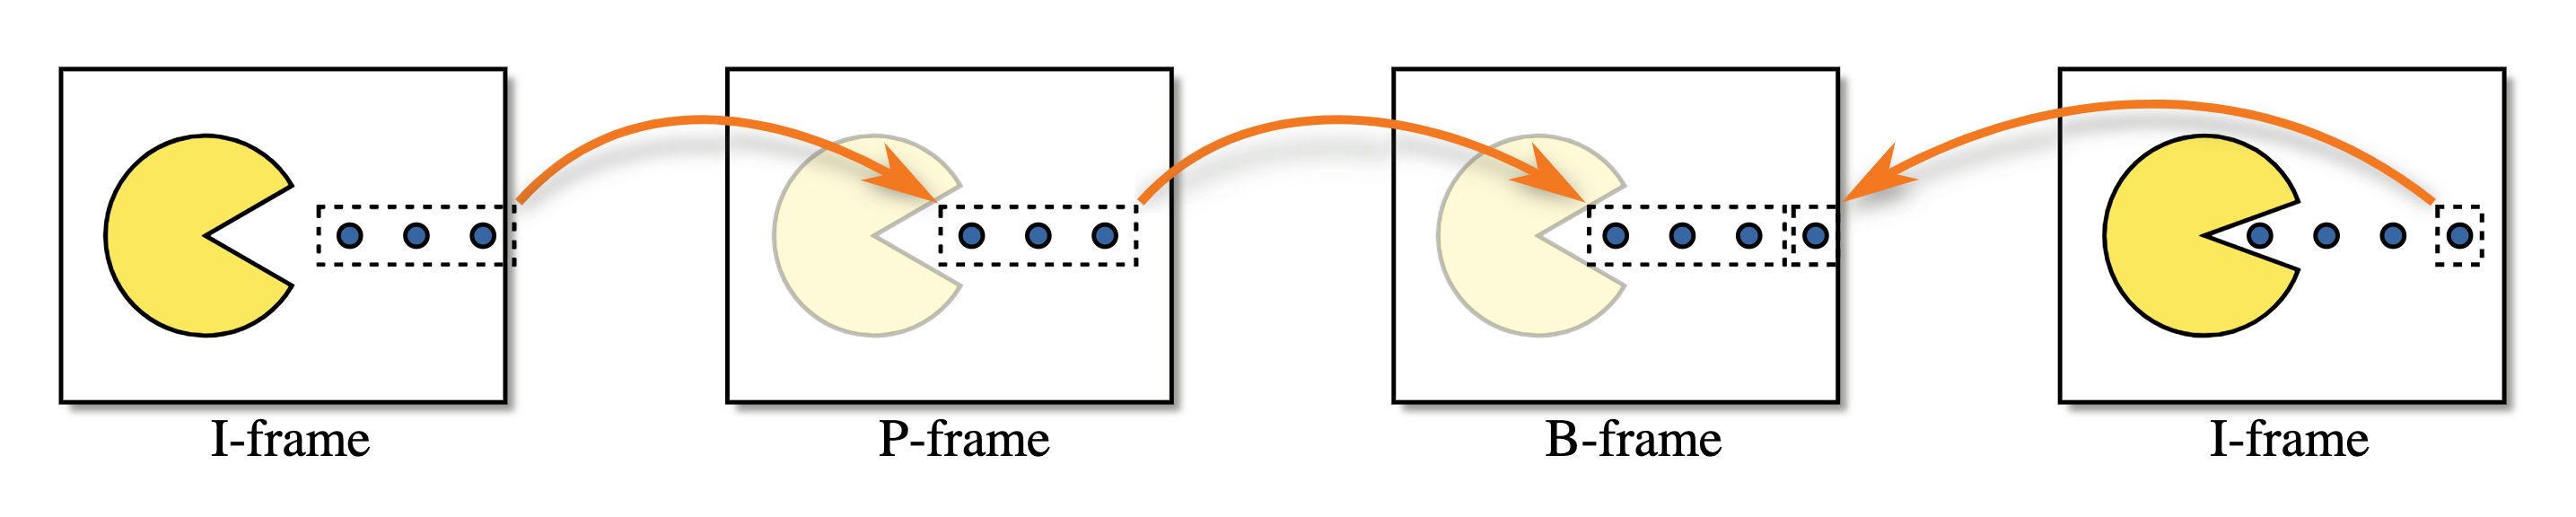
\includegraphics{images/frame_types.png}
}

\caption{
\label{frame-types}
     Типы кадров}
\end {center}
\end {figure}

\subsection{Потеря изображения}

Для решения проблемы с потерей изображения используются сообщения FIR (Full Intra Request) и PLI (Picture Loss Indication). Эти сообщения запрашивают у отправителя полный ключевой кадр.

PLI используется, когда декодер получает частичные кадры и не модет их декодировать. Такое может произойти при потере данных или ошибки декодера.

FIR не должен использоваться при потере пакетов или кадров согласно RFC 5104. FIR запрашивает ключевой кадр, например, при подключении к сессии нового участника, так как для начала декодирования видео требуется ключевой кадр, до его получения декодер будет отклонять остальные кадры \cite{v16}.

\pagebreak

% Scaling в файле scaling.tex
\specialsection{Масштабирование участников видеоконференций}

Хотя WebRTC представляет собой мощный интрумент для решения многих проблем при создании системы видеоконференций - он не идеален. Фреймворк WebRTC был разработан с учетом одноранговой (P2P) архитектуры, такой подход имеет проблемы с масштабируюмостью, если мы хотим одновременное присутствие большого количества участников. В WebRTC общающиеся стороны должны кодировать отдельный поток для получателей. Таким образом, каждый получатель связан независимым и выделенным кодером на стороне отправителя. Для поддержки N участников конференции с помощью чистой Mesh сети потребуется N * (N - 1) / 2 каналов. То есть требования к пропускной способности устройств будет расти квадратично по отношению к числу участников видеоконференции, рис ~\ref{mesh} \cite{v17}.

\begin{figure}[ht]
\begin{center}
\scalebox{0.30}{
   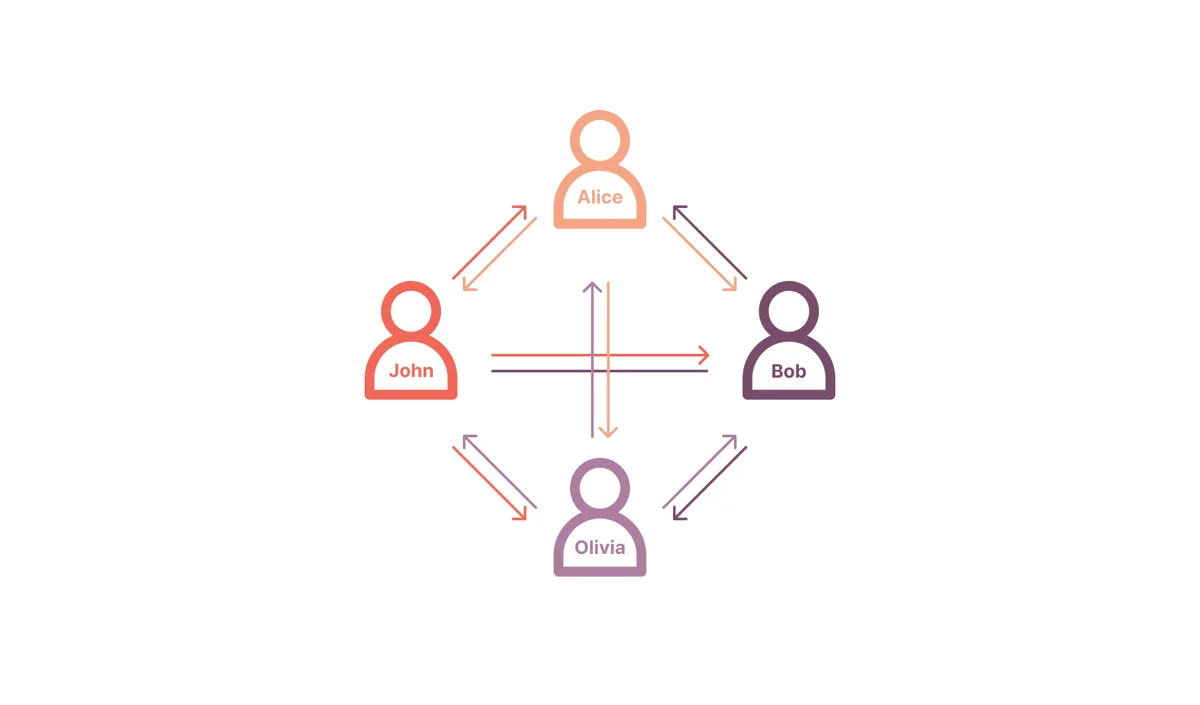
\includegraphics{images/mesh.png}
}

\caption{
\label{mesh}
     Mesh архитектура.}
\end {center}
\end {figure}

Чтобы улучшить масштабируемость этой архитектуры, можно использовать промежуточный медиасервер. В WebRTC есть 2 распространенных подхода - использование устройства многоточечной конференции (MCU) или устройства селективной переадресации (SFU).

\specialsubsection{SFU}

В WebRTC функции контроллера конференции может выполнять устройство селективной переадресации (SFU), задачей которого является получение всех потоков и принятие решения о том, какой поток должен быть отправлен какому участнику. Задача контроллера - оптимизация доставки потоков реального времени от отправителя к получателю.

В отличие от подхода MCU, SFU не требует декодирования/кодирования и поэтому является более легким. Его основная задача это принимать все потоки от участников и выборочно пересылать один или несколько потоков каждому получателю, рис. ~\ref{sfu}.

\begin{figure}[ht]
\begin{center}
\scalebox{0.50}{
   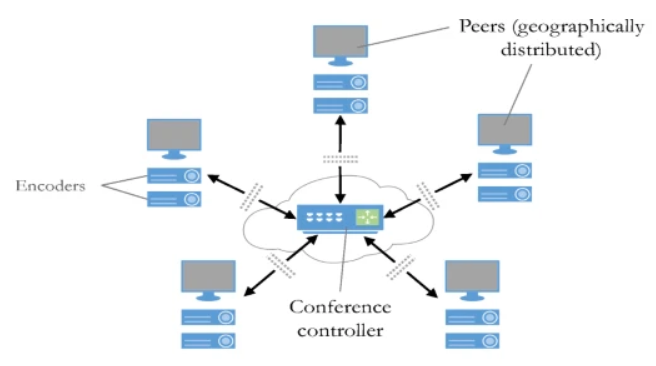
\includegraphics{images/sfu.png}
}

\caption{
\label{sfu}
     SFU архитектура.}
\end {center}
\end {figure}

При большом количестве участников количество пересылаемых потоков необходимо ограничивать, чтобы не тратить пропускную способность. По этой причине Грозева и др. разработали алгоритм идентификации докладчиков, который определит N последних доминирующих докладчиков конференции. Для экономии полосы пропускания только эти N потоков передаются участникам видеоконференции.

\begin{figure}[ht]
\begin{center}
\scalebox{0.50}{
   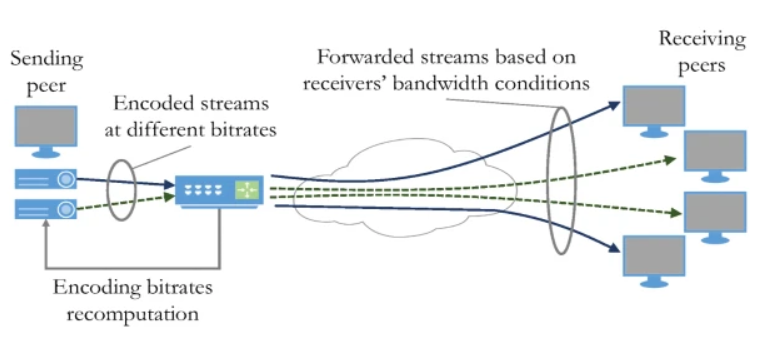
\includegraphics{images/sfu_forwarding.png}
}

\caption{
\label{sfu-forwarding}
     SFU controller dynamic forwarding.}
\end {center}
\end {figure}

По сути контроллер выполняет 2 основные задачи:
\begin{itemize}
	\item[1.] Получает все кодированные потоки от отправителя и динамически направляет их получателям, исходя из доступной пропускной способности, рис. ~\ref{sfu-forwarding};
	\item[2.] Переодически пересчитывает битрейты кодирования отправителя, чтобы лучше следовать долгосрочным колебаниям сети получателя \cite{v18}.
\end{itemize}

\specialsubsection{MCU}

Подход MCU заключается в том, чтобы получить все потоки от участников, декодировать и компилировать их в один общий поток, который отправляется обратно участникам. В итоге каждый участник должен отправлять и получать только один поток. Стоит понимать, что операции MCU дорогостоящие и требуют больших вычислительных затрат из процессов декодирования-смешивания-кодирования.

\begin{figure}[ht]
\begin{center}
\scalebox{0.90}{
   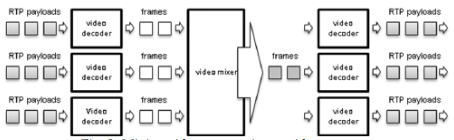
\includegraphics{images/mcu.png}
}

\caption{
\label{mcu}
     MCU смешивание аудиопотоков.}
\end {center}
\end {figure}

MCU назначает аудио/видео кодер и декодер, которые способны декодировать RTP-потоки от участников, кодер кодирует смешанные видеокадры обратно в полезную нагрузку RTP для каждого участника. Простое смешивание аудиопотоков всех участников в один поток привело бы к появлению эха от голоса. Чтобы этого избежать каждый участник должен иметь собственный аудиопоток, который не содержит его собственного звука. Сначала аудиокодеры декодируют полезную нагрузку RTP в аудиообразцы. Затем аудиомикшер смешивает аудиообразцы в отдельные потоки аудиообразцов, как показано на рис. ~\ref{mcu}. Потом отдельный аудиокодер кодирует аудиообразцы обратно в полезную нагрузку RTP \cite{v19}.

\specialsubsection{Сравнение архитектур}

\begin{center}
    \begin{longtable}{|p{4cm}|p{3cm}|p{3cm}|p{3cm}|}
    \caption{Сравнение Mesh, MCU, SFU архитектур.}\\
    \hline
     & Mesh & MCU & SFU\\ 
    \hline 
    in/out streams & 3/3 & 1/1 & 3/1\\
    \hline
    input traffic & 3 Мбит/с & 1 Мбит/с & 3 Мбит/с\\
    \hline
    output traffic & 3 Мбит/с & 1 Мбит/с & 1 Мбит/с\\
    \hline
    client CPU & 3 encoder + 3 decoder = 60\% & 1 encoder + 1 decoder = 20\% & 1 encoder + 3 decoder = 40\%\\
    \hline
    server CPU & 0 & 100\% & 10\%\\
    \hline
    latency & min & max & avg\\
    \hline
    SIP/live & -- & + & --\\
    \hline
    max participants & ~8 & $\infty$ & ~50\\
    \hline
    \end{longtable}
\end{center}

\specialsubsection{Mesh}

Mesh-топология выгодна за счет прямого соединения участников без вмешательства сервера, что сокращает издержки. 

Однако с ростом числа участников квадратично растет входящий и исходящий трафик. Создается большая нагрузка на CPU клиентского устройства, потому что большинство устройств поддерживают аппаратно ускоренное кодирование только одного потока в один момент, а тут надо кодировать и декодировать сразу несколько потоков.

\specialsubsection{MCU}

Основное преимущество MCU - число участников ограничено только количеством потоков, которое можно смикшировать на сервере. Кроме того, MCU экономит ресурсы на клиенте и позволяет реализовать трансляцию или запись на сервере.

Однако в MCU требуется много ресурсов на сервере, а также задержка в этой архитектуре самая большая.

\specialsubsection{SFU}

SFU архитектура выгодна за счет того, что часть нагрузки переносится с сервера на клиент. Кроме того исходящий трафик постоянен, а входящий растет пропорционально числу участников видеоконференции.

Главный минус SFU - это ограниченное число максимальных участников, которое, конечно, выше, чем в Mesh архитектуре, но меньше, чем в MCU. Это происходит из-за дорогого микширования входящих потоков, которое ложится на клиентов \cite{v20}.

\pagebreak

% Conclusion в файле conclusion.tex
\specialsection{ЗАКЛЮЧЕНИЕ}

В рамках этой научно-исследовательской работы мы рассмотрели историю развития видеоконференций, начиная с их зарождения в 1920-ых до современных технологий. Подробно рассмотрели протокол WebRTC и его возможности для обеспечения качественной коммуникации между участниками видеоконференций. Определили ожидания конечных пользователей и проблемы, влияющие на качество видеоконференций, а также рассмотрели, как WebRTC справляется с задачей передачи видео.

Одной из ключевых тем исследования было масштабирование участников видеоконференций. В частности, мы рассмотрели проблемы, связанные с ограничениями P2P архитектуры WebRTС и альтернативы, позволяющие решить проблему с масштабированием.

В будущих исследованиях мы подробно рассмотрим MCU (Multiple Control Unit) архитектуру для WebRTC, а также сосредоточимся на разработке и оптимизации приложения, устойчивого к условиям постоянного увеличения числа участников в видеоконференции.

\pagebreak

% Библиография в cpsconf стиле
% Аргумент {1} ниже включает переопределенный стиль с выравниванием слева
\begin{thebibliography}{1}
\bibitem{v1} The history and evolution of video conferencing. URL: \url{https://www.techtarget.com/whatis/feature/The-history-and-evolution-of-video-conferencing} (дата обращения: 21.05.2024).
\bibitem{v2} L. De Cicco, G. Carlucci and S. Mascolo, "Congestion Control for WebRTC: Standardization Status and Open Issues," in IEEE Communications Standards Magazine, vol. 1, no. 2, pp. 22-27, 2017, doi: 10.1109/MCOMSTD.2017.1700014.
\bibitem{v3} WebRTC for the Curious. What, Why and How. URL: \url{https://webrtcforthecurious.com/docs/01-what-why-and-how/} (дата обращения: 21.05.2024).
\bibitem{v4} Видеозвонки под капотом: от миллионов в сутки до 100 участников в одной конференции. URL: \url{https://habr.com/ru/companies/odnoklassniki/articles/479852} (дата обращения: 21.05.2024).
\bibitem{v5} BWE (Bandwidth Estimation). URL: \url{https://bloggeek.me/webrtcglossary/bwe/} (дата обращения: 21.05.2024).
\bibitem{v6} REMB (Receiver Estimated Maximum Bitrate). URL: \url{https://bloggeek.me/webrtcglossary/remb/} (дата обращения: 21.05.2024).
\bibitem{v7} TWCC (Transport Wide Congestion Control). URL: \url{https://bloggeek.me/webrtcglossary/transport-cc/} (дата обращения: 21.05.2024).
\bibitem{v8} Packet loss concealment. URL: \url{https://en.wikipedia.org/wiki/Packet_loss_concealment} (дата обращения: 21.05.2024).
\bibitem{v9} Packet Loss. URL: \url{https://bloggeek.me/webrtcglossary/packet-loss/} (дата обращения: 21.05.2024).
\bibitem{v10} FEC (Forward Error Correction). URL: \url{https://bloggeek.me/webrtcglossary/fec/} (дата обращения: 21.05.2024).
\bibitem{v11} Перегрузка сети. URL: \url{https://ru.wikipedia.org/wiki/%D0%9F%D0%B5%D1%80%D0%B5%D0%B3%D1%80%D1%83%D0%B7%D0%BA%D0%B0_%D1%81%D0%B5%D1%82%D0%B8} (дата обращения: 21.05.2024).
\bibitem{v12} Jitter. URL: \url{https://bloggeek.me/webrtcglossary/jitter/} (дата обращения: 21.05.2024).
\bibitem{v13} WebRTC for the Curious. Real-time Networking. URL: \url{https://webrtcforthecurious.com/docs/05-real-time-networking/} (дата обращения: 21.05.2024).
\bibitem{v14} MTU size. URL: \url{https://bloggeek.me/webrtcglossary/mtu-size/} (дата обращения: 21.05.2024).
\bibitem{v15} T. Beneš, S. Ubik and J. Halák, "Packet Reordering Correction for Low-Latency Network Applications," 2022 11th Mediterranean Conference on Embedded Computing (MECO), Budva, Montenegro, 2022, pp. 1-5, doi: 10.1109/MECO55406.2022.9797070.
\bibitem{v16} WebRTC for the Curious. Media Communication. URL: \url{https://webrtcforthecurious.com/docs/06-media-communication/} (дата обращения: 21.05.2024).
\bibitem{v17} 
WebRTC Video API
Understanding P2P, SFU, and MCU WebRTC Architectures. URL: \url{https://www.digitalsamba.com/blog/p2p-sfu-and-mcu-webrtc-architectures-explained} (дата обращения: 21.05.2024).
\bibitem{v18} Stefano Petrangeli, Dries Pauwels, Jeroen Van Der Hooft, Matúš ?Iak, Jürgen Slowack, Tim Wauters, and Filip De Turck. 2019. A scalable WebRTC-based framework for remote video collaboration applications. Multimedia Tools Appl. 78, 6 (March 2019), 7419–7452. https://doi.org/10.1007/s11042-018-6460-0.
\bibitem{v19} Ng, Kwok \& Ching, Man \& Liu, Yang \& Cai, Tao \& Li, Li \& Chou, Wu. (2014). A P2P-MCU Approach to Multi-Party Video Conference with WebRTC. International Journal of Future Computer and Communication. 3. 319-324. 10.7763/IJFCC.2014.V3.319.
\bibitem{v20} Как это устроено: видеоконференции ВКонтакте на безлимитное число участников. URL: \url{https://habr.com/ru/companies/vk/articles/575358/} (дата обращения: 21.05.2024).
\bibitem{v21} WebRTC for the Curious. Signaling. URL: \url{https://webrtcforthecurious.com/docs/02-signaling/} (дата обращения: 21.05.2024).
\bibitem{v22} WebRTC for the Curious. Connecting. URL: \url{https://webrtcforthecurious.com/docs/03-connecting/} (дата обращения: 21.05.2024).
\bibitem{v23} WebRTC for the Curious. Securing. URL: \url{https://webrtcforthecurious.com/docs/04-securing/} (дата обращения: 21.05.2024).
\bibitem{v24} WebRTC for the Curious. Data Communication. URL: \url{https://webrtcforthecurious.com/docs/07-data-communication/} (дата обращения: 21.05.2024).
\bibitem{v25} Что такое STUN-сервер? URL: \url{https://www.3cx.ru/voip-sip/stun-server/} (дата обращения: 21.05.2024).
\bibitem{v26} STUN: Definition and explanation. URL: \url{https://bloggeek.me/webrtcglossary/stun/} (дата обращения: 21.05.2024).
\bibitem{v27} Обзор протоколов STUN, TURN и ICE, их принципы работы с NAT и использование для VoIP. URL: \url{https://voxlink.ru/kb/asterisk-configuration/obzor-protokolov-stun-turn-i-ice-ih-principy-raboty-s-nat-i-ispolzovanie-dlja-voip/} (дата обращения: 21.05.2024).
\end{thebibliography}
\end{document}